\documentclass{article}
\usepackage[utf8]{inputenc}
\usepackage{authblk}
\usepackage[margin=1.7in]{geometry}
\usepackage{wrapfig}
\usepackage{graphicx}

\title{Data Aggregation \& Analysis System for Intelligent Agriculture: Design Document}
\author[1]{Panagiotis Stanitsas \thanks{stani078@umn.edu}}
\author[1]{Jacob Quant \thanks{quant006@umn.edu}}
\author[1]{Nabil Cheikh  \thanks{cheik004@d.umn.edu}}
% TODO: Don't forget to put "Team ID 1" somewhere on here
% TODO: Do you think we should include the course or section number also?
	
\affil[1]{Department of Computer Science and Engineering, University of Minnesota, Minneapolis, MN 55455 USA}

\renewcommand\Authands{ and }
\date{}

\begin{document}

\maketitle

%\begin{abstract}
%\end{abstract}

\section{Motivation}
Over the past decade a great amount of attention has been received in the area of intelligent system development in precision agriculture. Methods along the lines of satellite and drone image processing as well as technologically advanced sensing techniques are deployed in an effort to increase the efficiency of modern crops while optimizing the quantities of the necessary resources (e.g. fertilizers, water). Figure \ref{fig:HighLev} 

% TODO: Photo credit?
\begin{wrapfigure}{l}{3in}
\begin{center}
   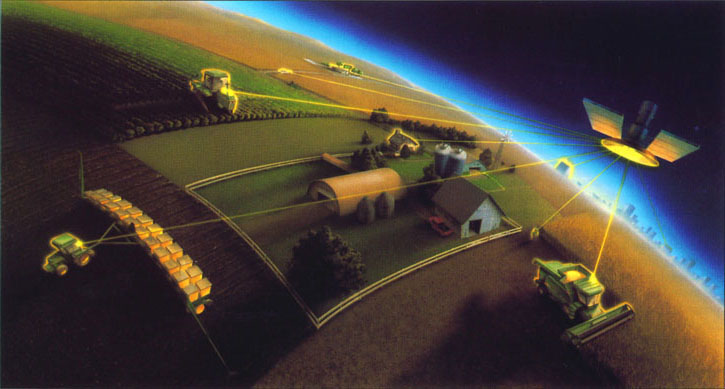
\includegraphics[width=1\linewidth,trim={0 0 0 0cm},clip]{Images/HighLevel.jpg}
\end{center}
\vspace{-0.2in}
   \caption{\footnotesize{A High-Level Overview of Precision Agriculture.}}
   \label{fig:HighLev}
   %\vspace{-0.08in}
\end{wrapfigure}

\noindent illustrates a high-level view of the the multistage structure of modern Precision Agriculture according to which information is aggregated at a central hub, then processed and based on the results, all agents receive a plan of action regarding irrigation, fertilization, harvesting and planting.  Capitalizing on the continuous effort of reducing the associated cost with Precision Agriculture applications, cheap sensing solutions can be implemented in order to provide valuable information even on the farmer's smart phones. In particular, the scenario that this project aims to replicate is the delivery of information, which is harvested in the field, to a mobile device based on user defined queries. Sensors that can measure the humidity of the soil can be purchased at a very low price (\$10 - \$20), 
\begin{wrapfigure}{r}{2.0in}
\begin{center}
   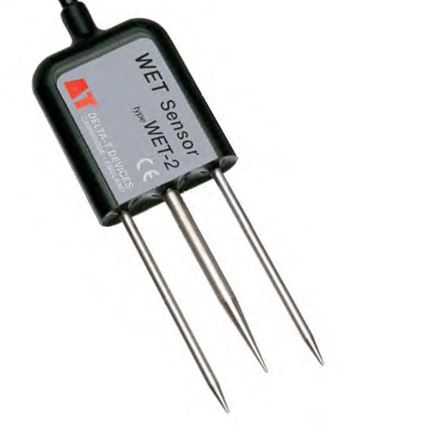
\includegraphics[width=1\linewidth,trim={0 0 0 0cm},clip]{Images/HumSens.jpg}
\end{center}
\vspace{-0.2in}
   \caption{Soil humidity sensor}
   \label{fig:Humsens}
   %\vspace{-0.08in}
\end{wrapfigure}

\noindent while constructing a wireless network (e.g. ZigBee modules) that is capable of transmitting
the sensor measurements to a central processing location can be also completed within a constricted budget.
Figure \ref{fig:Humsens} presents a soil humidity sensor distributed by Hoskin Scientific and has the ability to measure water content and temperature directly within the root zone. Rather than using sophisticated devices to deliver information to the farmer, this effort promotes the use of a phone application user while remaining aligned with the initial goal of keeping the cost as low as possible. In that way, utilizing low-cost sensor measurements, farmers can monitor the humidity (of the soil) and plan accordingly for their irrigation strategies.


\section{Implementation Outline}

In summary, our team intends to develop an Android application, capable of delivering heat-map visualizations of humidity and temperature (if time allows) time series for user defined locations and time periods. 

The proposed methodology has three discrete components. The first, is concerned with the sensors’ deployment as well as the collection of measurements in the field. For the purposes of this study data will be simulated using appropriately selected random number generators since the time-frame does not allow experimentation with those hardware components as well. The second component includes multiple modules and refers to tasks that the server needs to perform. Three modules are associated with the server’s component: a collection and storage module, a data analysis and visualization module, and a module to process requests received from the end-user using these other modules. The last component is the client application, which runs on an Android device and is responsible for submitting the user’s queries and displaying the results. 
Figure \ref{fig:module-relationships} illustrates the relationships among the different components of this system.

\begin{figure*}[htb]
\begin{center}
   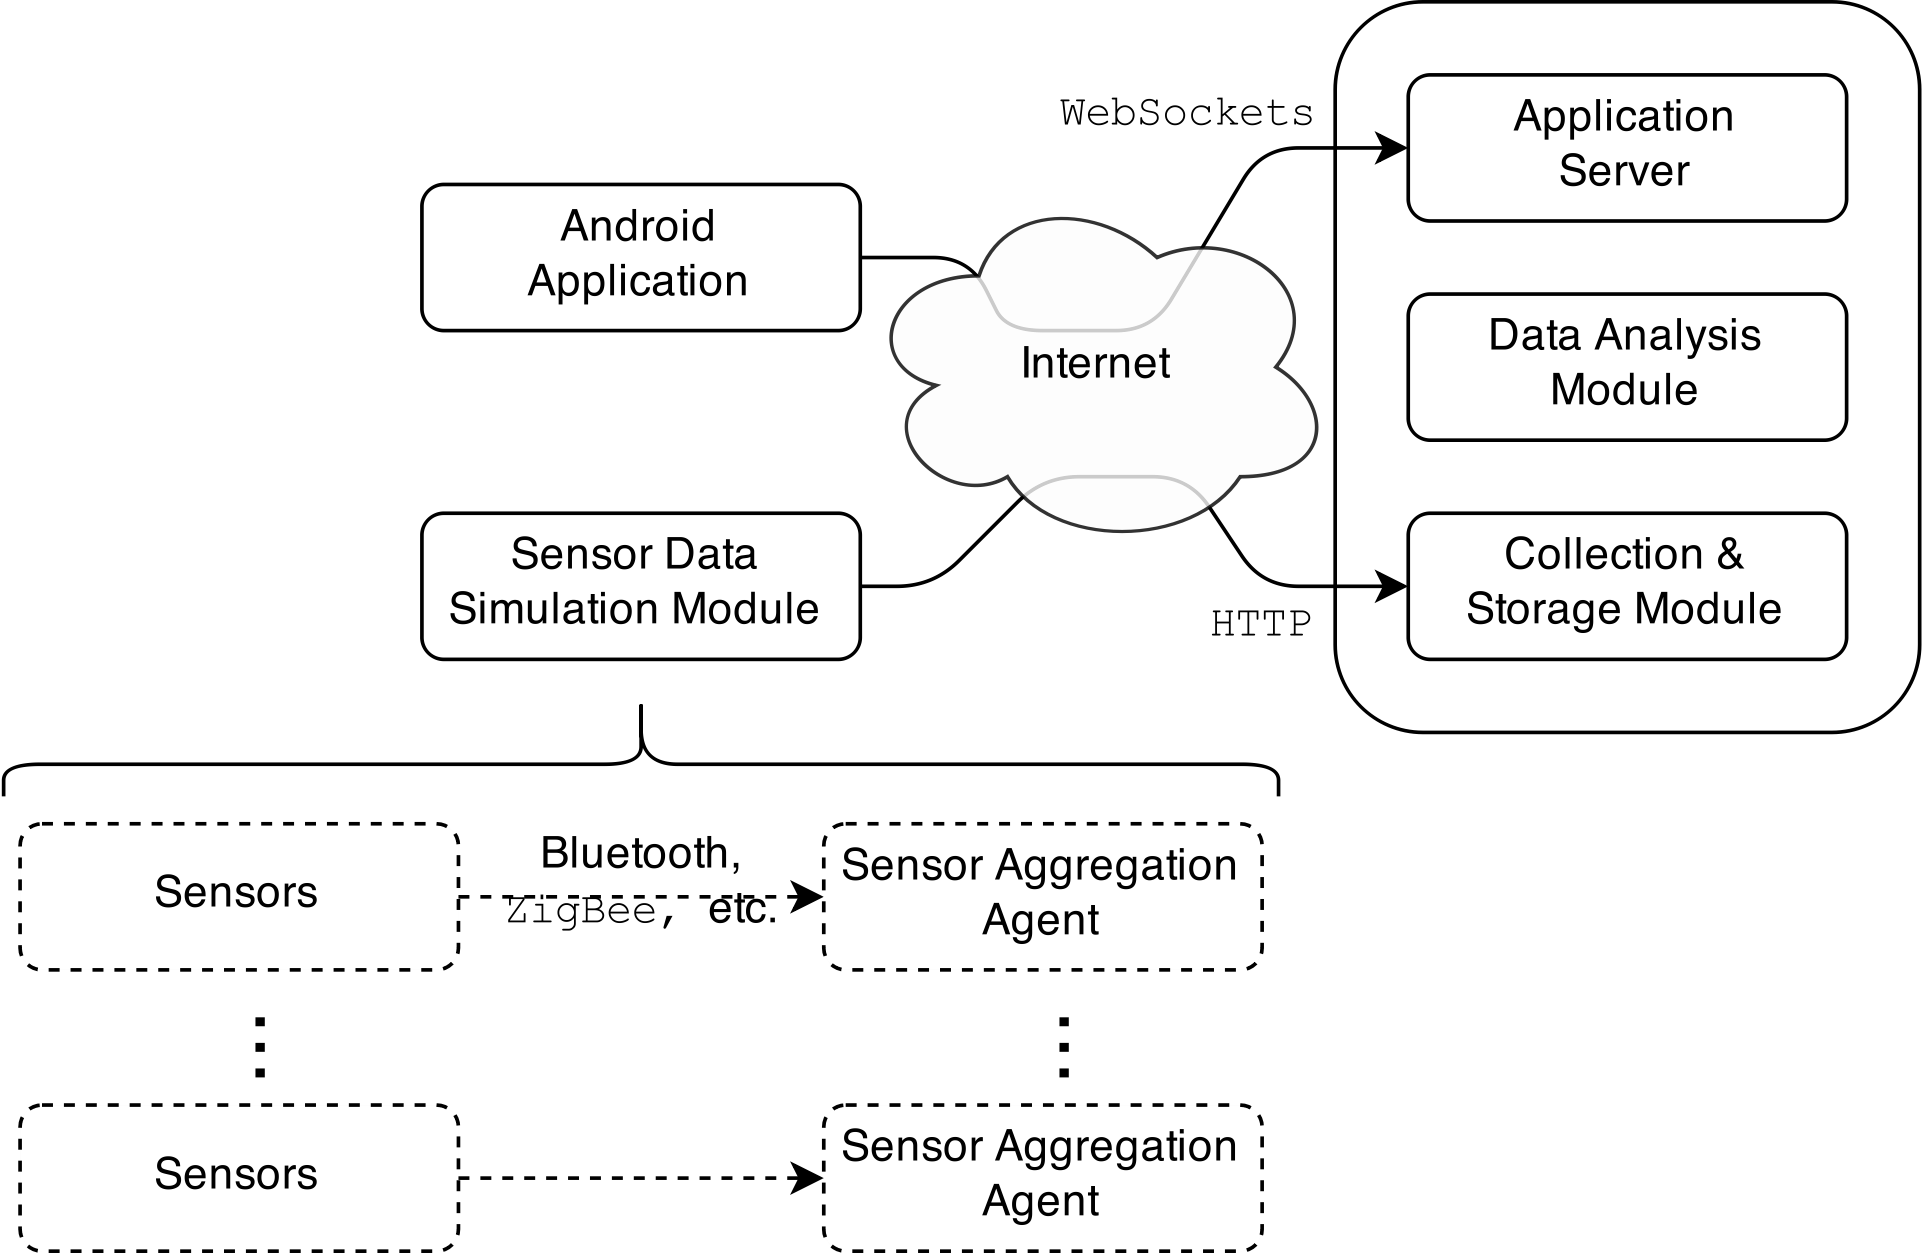
\includegraphics[width=1\linewidth]{Images/module-relationships.png}
\end{center}
\vspace{-0.2in}
   \caption{Component relationships (dashed borderlines indicate portions that are out of scope)}
   \label{fig:module-relationships}
   %\vspace{-0.08in}
\end{figure*}


% TODO: If we're going to include a relevant/related work section, wouldn't it make more sense
% to place it before the implementation outline (i.e. closer the motivation/introduction/abstract)?
%\section{Relevant work}

% These sections will go into more detail about each of the components
% Client/App/Front-end <--> Server <--> Analysis <--> Storage <--> Sensors (simulator)
\section{Implementation Details}
The sections that follow go into more detail about how each component in this system
accomplishes its function. 

\subsection{Sensor Data Simulator}
In lieu of physical sensors collecting ``real world'' measurements,
this module simulates a collection of virtual sensors.
For each dimension (e.g. moisture content, temperature, etc.), rather than simply
generating random, independent values for each sensor at each sample time
we want to generate more realistic data.
To do this, we define a consistent model that takes into consideration both
the time of the measurement (e.g. daily temperature cycles and seasonal variation) and
the location of the sensor (e.g. perhaps some portion of the region being modeled has a lower elevation or less permeable soil).
We may also feed a set of historic weather data through the simulator.
Perhaps the most important aspect of this component is not so much that it generate meaningful data
but rather that it be replaceable by a system of real sensors without any disruption to the downstream
components that process its output.

The format 


\subsection{Storage Module}


\begin{figure*}[htb]
\begin{center}
   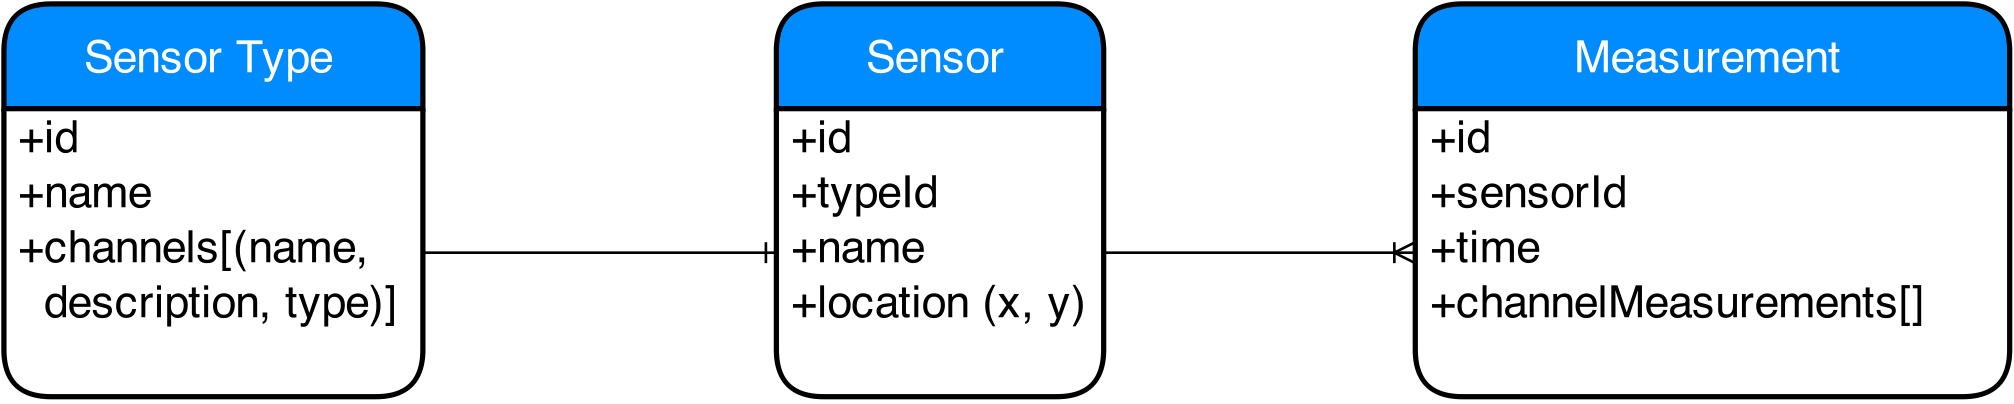
\includegraphics[width=1\linewidth]{Images/DB-Schema.png}
\end{center}
\vspace{-0.2in}
   \caption{"Soft" database schema}
   \label{fig:db-soft-schema}
   %\vspace{-0.08in}
\end{figure*}


\subsection{Data Analysis Module}

The Data Analysis Module (DAM) will be written in Python and will be responsible for analyzing the data that correspond to the user's request. The \textbf{input} to this module is a 3D array of dimensions $\mathbf{Nx3xT}$ where $\mathbf{N}$ is the number of sensors in the user defined region of interest and $\mathbf{T}$ is the number of time frames that the user requested. For each sensor and each time-frame its x-y coordinates along with the harvested measuremnt are provided.

Two blocks can be identified in the intended implementation of this module. The first block is responsible for solving a 2D interpolation problem for which the locations of a small number of point measurements are available and an estimate about the humidity conditions across a larger grid of points needs to be computed. 

During this preliminary investigation phase the \tekriging method for interpolating spatial data was tested; the computational complexity of the kriging method makes it a bad candidate for the targeted implementation. Even though it is a very accurate method for this task, a simpler implementation using multiple 2D Gaussian distributions centered at the locations that measurements are available is more appropriate. Figure \ref{fig:Analytics} (a) presents 5 Gaussian distributions placed on a 2D grid emulating the  aforementioned scenario, thus the case of having 5 sensors. Figure \ref{fig:Analytics} (b) presents an existing implementation that superimposes the computed heatmap on GoogleMaps for better visualization. If time allows this feature will also become available in our implementation. 

\begin{figure*}[!htbp]
\begin{center}
\begin{tabular}{c c}
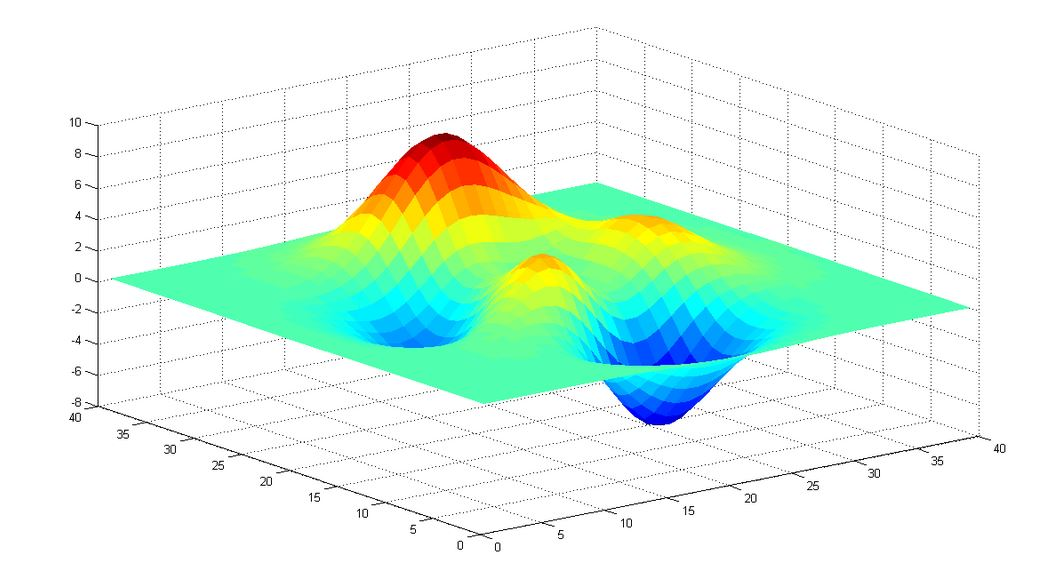
\includegraphics[width=0.45\linewidth]{Images/multipleGaus.jpg}&
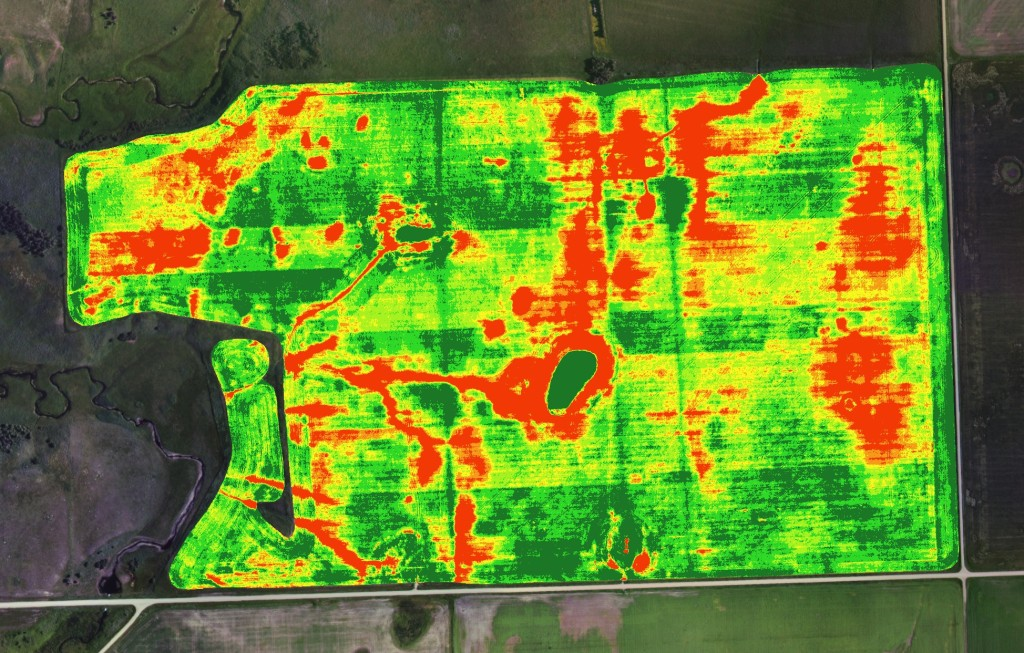
\includegraphics[width=0.45\linewidth]{Images/HeatMap.jpg}\\
(a) & (b)
\end{tabular}
\end{center}
\vspace{-0.15in}
\caption{\label{fig:Analytics} {\footnotesize (a) 5 Gaussian distributions placed on a 2D grid. (b) Superimposing the heat map on the GoogleMaps. }}
%\vspace{-0.08in}
\end{figure*}

The second block of this module is responsible for harvesting the $\mathf{T}$ heatmaps generated in the above implementation and returns a video object. The implementation of this task will be performed using the \textbf{Python Imaging Libray} and the output will be 
\subsection{Server}

\subsection{Front-end}





\section{Module Aggregation}



\end{document}
